\documentclass[11pt]{article}
\usepackage{colacl06}
\usepackage{times,url}
\usepackage{latexsym}
\usepackage{hyphen}
\usepackage{epsfig}
\setlength\titlebox{6.5cm}    % Expanding the titlebox

\title{NLTK: The Natural Language Toolkit}

\author{Steven Bird\\[.5ex]
  Department of Computer Science and Software Engineering\\
  University of Melbourne, Victoria 3010, AUSTRALIA\\[.5ex]
  Linguistic Data Consortium, University of Pennsylvania,\\
  Philadelphia PA 19104-2653, USA}
\date{}

\begin{document}
\maketitle
\begin{abstract}
  The Natural Language Toolkit is a suite of program modules, data
  sets and tutorials supporting research and teaching in computational
  linguistics and natural language processing.  NLTK is written in
  Python and distributed under the GPL open source license.  Over the
  past year the toolkit has been rewritten, simplifying many
  linguistic data structures and taking advantage of recent
  enhancements in the Python language.  This paper reports on the
  simplified toolkit and explains how it is used in teaching NLP.
\end{abstract}

\section{Introduction}

NLTK, the Natural Language Toolkit, is a suite of Python modules
providing many NLP data types, processing tasks, corpus samples and
readers, together with animated algorithms, tutorials, and problem
sets \cite{LoperBird02}.  Data types include tokens, tags, chunks,
trees, and feature structures.  Interface definitions and reference
implementations are provided for tokenizers, stemmers, taggers
(regexp, ngram, Brill), chunkers, parsers (recursive-descent,
shift-reduce, chart, probabilistic), clusterers, and classifiers.
Corpus samples and readers include: Brown Corpus, CoNLL-2000 Chunking
Corpus, CMU Pronunciation Dictionary, NIST IEER Corpus, PP Attachment
Corpus, Penn Treebank, and the SIL Shoebox corpus format.

NLTK is ideally suited to students who are learning NLP or conducting
research in NLP or closely related areas.
NLTK has been used successfully as a
teaching tool, as an individual study tool, and as a platform for
prototyping and building research systems \cite{Liddy05,Satre05}.

We chose Python for its shallow learning curve, transparent syntax,
and good string-handling.  Python permits exploration via its
interactive interpreter.  As an object-oriented language, Python
permits data and code to be encapsulated and re-used easily.  Python
comes with an extensive library, including tools for graphical
programming and numerical processing \cite{Beasley06}.

Over the past four years the toolkit grew rapidly and the data
structures became significantly more complex.  Each new processing
task added new requirements on input and output
representations.  It was not clear how to generalize tasks so they
could be applied independently of each other.

As a simple example, consider the independent tasks of tagging and
stemming, which both operate on sequences of tokens.  If stemming is
done first, we lose information required for tagging.  If tagging is
done first, the stemming must be able to skip over the tags.  If both
are done independently, we need to be able to align the results.  As
task combinations multiply, managing the data becomes extremely
difficult.

To address this problem, NLTK 1.4 introduced a blackboard architecture
for tokens, unifying many data types, and permitting distinct tasks to
be run independently.  Unfortunately this architecture also came with
a significant overhead for programmers, who were often forced to use
``rather awkward code structures'' \cite{Hearst05}.  It was clear that
the re-engineering done in NLTK 1.4 unduly complicated the
programmer's task.

This paper presents a brief overview and tutorial on a new, simplified
toolkit, and describes how it is used in teaching.

\section{Simple Processing Tasks}

\subsection{Tokenization and Stemming}

The following three-line program imports the \texttt{tokenize}
package, defines a text string, and tokenizes the string on
whitespace to create a list of tokens.  (NB.\ `\url{>>>}' is
Python's interactive prompt; `\url{...}' is the continuation prompt.)

{\small\begin{verbatim}
>>> text = 'This is a test.'
>>> list(tokenize.whitespace(text))
['This', 'is', 'a', 'test.']
\end{verbatim}}

\noindent
Several other tokenizers are provided.  We can stem the output of tokenization
using the Porter Stemmer as follows:

{\small\begin{verbatim}
>>> text = 'stemming is exciting'
>>> tokens = tokenize.whitespace(text)
>>> porter = stem.Porter()
>>> for token in tokens:
...     print porter.stem(token),
stem is excit
\end{verbatim}}

The corpora included with NLTK come with corpus readers that
understand the file structure of the corpus, and load the data into
Python data structures.  For example, the following code reads part \textit{a}
of the Brown Corpus.  It prints a list of tuples, where each tuple
consists of a word and its tag.

{\small\begin{verbatim}
>>> for sent in brown.tagged('a'):
...     print sent
[('The', 'at'), ('Fulton', 'np-tl'),
('County', 'nn-tl'), ('Grand', 'jj-tl'),
('Jury', 'nn-tl'), ('said', 'vbd'), ...]
\end{verbatim}}

NLTK provides support for conditional frequency distributions, making
it easy to count up items of interest in specified contexts.  Such
information may be useful for studies in stylistics or in text
categorization.

\subsection{Tagging}

The simplest possible tagger assigns the same tag to each token:

{\small\begin{verbatim}
>>> my_tagger = tag.Default('nn')
>>> list(my_tagger.tag(tokens))
[('John', 'nn'), ('saw', 'nn'),
 ('3', 'nn'), ('polar', 'nn'),
 ('bears', 'nn'), ('.', 'nn')]
\end{verbatim}}

On its own, this will tag only 10--20\% of the tokens correctly.
However, it is a reasonable tagger to use as a default if a more
advanced tagger fails to determine a token's tag.

The regular expression tagger assigns a tag to a token according to a
series of string patterns.  For instance, the following tagger assigns
\texttt{cd} to cardinal numbers, \texttt{nns} to words ending in the
letter \textit{s}, and \texttt{nn} to everything else:

{\small\begin{verbatim}
>>> patterns = [
...     (r'\d+(.\d+)?$', 'cd'),
...     (r'\.*s$', 'nns'),
...     (r'.*', 'nn')]
>>> simple_tagger = tag.Regexp(patterns)
>>> list(simple_tagger.tag(tokens))
[('John', 'nn'), ('saw', 'nn'),
 ('3', 'cd'), ('polar', 'nn'),
 ('bears', 'nns'), ('.', 'nn')]
\end{verbatim}}
    
The \texttt{tag.Unigram} class implements a simple statistical tagging
algorithm: for each token, it assigns the tag that is most likely
for that token. For example, it will assign the tag \texttt{jj} to
any occurrence of the word \textit{frequent}, since \textit{frequent} is used as an
adjective (e.g.\ \textit{a frequent word}) more often than it is used as a
verb (e.g.\ \textit{I frequent this cafe}).
Before a unigram tagger can be used, it must be trained on
a corpus, as shown below for the first section of the Brown Corpus.

{\small\begin{verbatim}
>>> unigram_tagger = tag.Unigram()
>>> unigram_tagger.train(brown('a'))
\end{verbatim}}
    
\noindent
Once a unigram tagger has been trained, it can be used to tag new text.
Note that it assigns the default tag \texttt{None} to any token that was not
encountered during training.

{\small\begin{verbatim}
>>> text = "John saw the books on the table"
>>> tokens = list(tokenize.whitespace(text))
>>> list(unigram_tagger.tag(tokens))
[('John', 'np'), ('saw', 'vbd'),
 ('the', 'at'), ('books', None),
 ('on', 'in'), ('the', 'at'),
 ('table', None)]
\end{verbatim}}
    
\noindent
We can instruct the unigram tagger to back off to our default
\url{simple_tagger} when it cannot assign a tag itself.  Now all
the words are guaranteed to be tagged:

{\small\begin{verbatim}
>>> unigram_tagger =
...     tag.Unigram(backoff=simple_tagger)
>>> unigram_tagger.train(train_sents)
>>> list(unigram_tagger.tag(tokens))
[('John', 'np'), ('saw', 'vbd'),
 ('the', 'at'), ('books', 'nns'),
 ('on', 'in'), ('the', 'at'),
 ('table', 'nn')]
\end{verbatim}}

\noindent
We can go on to define and train a bigram tagger, as shown below:

{\small\begin{verbatim}
>>> bigram_tagger =\
...     tag.Bigram(backoff=unigram_tagger)
>>> bigram_tagger.train(brown.tagged('a'))
\end{verbatim}}

\noindent
We can easily evaluate this tagger against some gold-standard tagged
text, using the \url{tag.accuracy()} function.

NLTK also includes a Brill tagger (contributed by Christopher
Maloof) and an HMM tagger (contributed by Trevor Cohn).

\section{Chunking and Parsing}

Chunking is a technique for shallow syntactic analysis of (tagged)
text.  Chunk data can be loaded from files that use the common bracket or
IOB notations.  We can define a regular-expression based chunk parser
for use in chunking tagged text.  NLTK also supports simple cascading
of chunk parsers.  Corpus readers for chunked data in Penn Treebank
and CoNLL-2000 are provided, along with comprehensive support for
evaluation and error analysis.

NLTK provides several parsers for context-free phrase-structure
grammars.  Grammars can be defined using a series of productions as follows:

{\small\begin{verbatim}
>>> grammar = cfg.parse_grammar('''
...     S -> NP VP
...     VP -> V NP | V NP PP
...     V -> "saw" | "ate"
...     NP -> "John" | Det N | Det N PP
...     Det -> "a" | "an" | "the" | "my"
...     N -> "dog" | "cat" | "ball"
...     PP -> P NP
...     P -> "on" | "by" | "with"
...     ''')
\end{verbatim}}

\noindent
Now we can tokenize and parse a sentence with a recursive descent
parser.  Note that we avoided left-recursive productions in the above
grammar, so that this parser does not get into an infinite loop.

{\small\begin{verbatim}
>>> text = "John saw a cat with my ball"
>>> sent = list(tokenize.whitespace(text))
>>> rd = parse.RecursiveDescent(grammar)
\end{verbatim}}

Now we apply it to our sentence, and iterate over all the parses that
it generates.  Observe that two parses are possible, due to
prepositional phrase attachment ambiguity.

{\small\begin{verbatim}
>>> for p in rd.get_parse_list(sent):
...     print p
(S:
  (NP: 'John')
  (VP:
    (V: 'saw')
    (NP:
      (Det: 'a')
      (N: 'cat')
      (PP: (P: 'with')
        (NP: (Det: 'my') (N: 'ball'))))))
(S:
  (NP: 'John')
  (VP:
    (V: 'saw')
    (NP: (Det: 'a') (N: 'cat'))
    (PP: (P: 'with')
      (NP: (Det: 'my') (N: 'ball')))))
\end{verbatim}}

\noindent
The same sentence can be parsed using a grammar with left-recursive
productions, so long as we use a chart parser.  We can invoke NLTK's
chart parser with a bottom-up rule-invocation strategy with
\texttt{chart.ChartParse(grammar, chart.BU$\_$STRATEGY)}.  Tracing can
be turned on in order to display each step of the process.  NLTK also
supports probabilistic context free grammars, and provides a
Viterbi-style PCFG parser, together with a suite of bottom-up
probabilistic chart parsers.

\begin{figure*}[tb]
\centerline{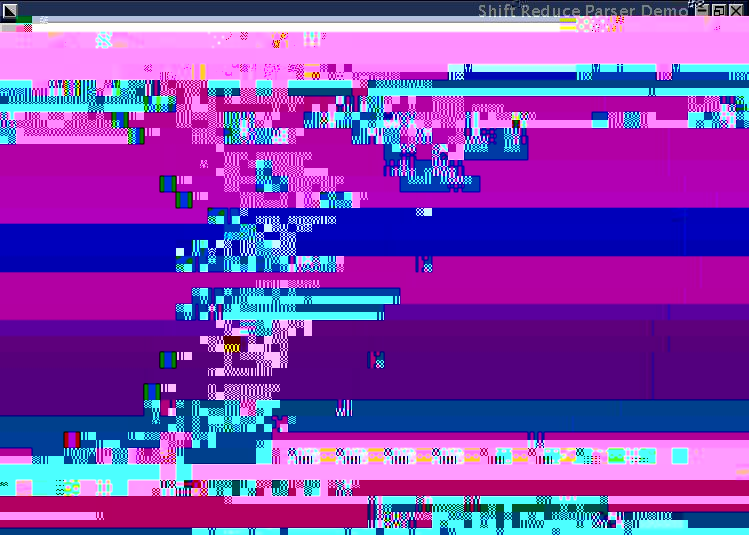
\epsfig{file=srparser.eps, scale=.5}}
\vspace{4ex}
\centerline{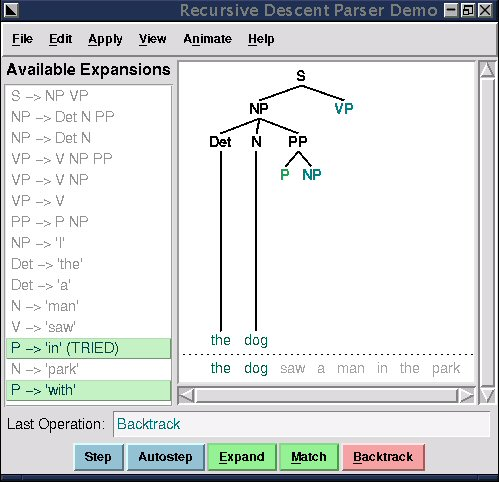
\epsfig{file=rdparser.eps, scale=.5}}
\caption{Two Parser Demonstrations: Shift-Reduce and Recursive Descent Parsers}
\label{fig:parser}
\end{figure*}
\section{Teaching with NLTK}

Natural language processing is often taught within the confines of a
single-semester course, either at advanced undergraduate level or at
postgraduate level.  Unfortunately, it turns out to be rather
difficult to cover both the theoretical and practical sides of the
subject in such a short span of time.  Some courses focus on theory to
the exclusion of practical exercises, and deprive students of the
challenge and excitement of writing programs to automatically process
natural language.  Other courses are simply designed to teach
programming for linguists, and do not manage to cover any significant
NLP content.  NLTK was developed to address this problem, making
it feasible to cover a substantial amount of theory and practice
within a single-semester course.

A significant fraction of any NLP course is made up of fundamental
data structures and algorithms.  These are usually taught with the
help of formal notations and complex diagrams.  Large trees and charts
are copied onto the board and edited in tedious slow motion, or
laboriously prepared for presentation slides.  A more effective method
is to use live demonstrations in which those diagrams are generated
and updated automatically.  NLTK provides interactive graphical user
interfaces, making it possible to view program state and to study
program execution step-by-step (e.g.\ see Figure~\ref{fig:parser}).
Most NLTK components have a demonstration mode, and will perform an
interesting task without requiring any special input from the user.
It is even possible to make minor modifications to programs in
response to ``what if'' questions.  In this way, students learn the
mechanics of NLP quickly, gain deeper insights into the data
structures and algorithms, and acquire new problem-solving skills.
Since these demonstrations are distributed with the toolkit, students
can experiment on their own with the algorithms that they have seen
presented in class.

NLTK can be used to create student assignments of varying difficulty
and scope. In the simplest assignments, students experiment with one
of the existing modules.  Once students become more familiar with the
toolkit, they can be asked to make minor changes or extensions to an
existing module (e.g.\ build a left-corner parser by modifying the
recursive descent parser).  A bigger challenge is to develop one or
more new modules and integrate them with existing modules to perform
a sophisticated NLP task.  Here, NLTK provides a useful starting
point with its existing components and its extensive tutorials and
API documentation.

NLTK is a unique framework for teaching natural language processing.
NLTK provides comprehensive support for a first course in NLP which
tightly couples theory and practice.  Its extensive documentation
maximizes the potential for independent learning.  For more
information, including documentation, download pointers, and links to
dozens of courses that have adopted NLTK, please see:
\url{http://nltk.sourceforge.net/} .

\section*{Acknowledgements}

I am grateful to Edward Loper, co-developer of NLTK, and to dozens of
people who have contributed code and provided helpful feedback.
\vspace{-2ex}

\bibliographystyle{acl}

\begin{thebibliography}{}
\setlength{\parskip}{0pt}
\setlength{\itemsep}{0pt}

\bibitem[\protect\citename{Hearst}2005]{Hearst05}
Marti Hearst.
\newblock 2005.
\newblock Teaching applied natural language processing: Triumphs and
  tribulations.
\newblock In {\em Proc 2nd ACL Workshop on Effective Tools and
  Methodologies for Teaching NLP and CL}, pages 1--8, ACL

\bibitem[\protect\citename{Liddy and McCracken}2005]{Liddy05}
Elizabeth Liddy and Nancy McCracken.
\newblock 2005.
\newblock Hands-on {NLP} for an interdisciplinary audience.
\newblock In {\em Proc 2nd ACL Workshop on Effective Tools and
  Methodologies for Teaching NLP and CL}, pages 62--68, ACL

\bibitem[\protect\citename{Loper and Bird}2002]{LoperBird02}
Edward Loper and Steven Bird.
\newblock 2002.
\newblock {NLTK}: The Natural Language Toolkit.
\newblock In {\em Proc ACL Workshop on Effective Tools and
  Methodologies for Teaching Natural Language Processing and Computational
  Linguistics}, pages 62--69. ACL.

\bibitem[\protect\citename{Beasley}2006]{Beasley06}
David Beasley.
\newblock 2006.
\newblock {\em Python Essential Reference, 3rd Edition}.
\newblock Sams.

\bibitem[\protect\citename{S{\ae}tre \bgroup et al.\egroup }2005]{Satre05}
Rune S{\ae}tre, Amund Tveit, Tonje~S. Steigedal, and Astrid L{\ae}greid.
\newblock 2005.
\newblock Semantic annotation of biomedical literature using Google.
\newblock In {\em Data Mining and Bioinformatics Workshop}, volume 3482 of {\em
  Lecture Notes in Computer Science}. Springer.

\end{thebibliography}
\end{document}
